\section{Teori}
I detta kapitel ska det förklaras hur {\LaTeX} används för att 

\subsection{Språket {\LaTeX}} 
{\LaTeX} är ett bla bla finns till Linux, Mac och Windows.  
\newline
\newline
{\LaTeX} är ett programmeringsspråk vilket betyder att olika programmeringstekniker kan tillämpas. Ett exempel är top-down design där abstrakta funktioner kan defineras först för att sedan delas upp i mindre konkreta funktioner. I ett dokument kan det handla om att definiera strukturen först innan någon text är skriven. 
\newline
\newline
Det är ett Turing-komplett språk vilket låter användaren definera sina egna kommandon. Dessa kommandon kan användas för att göra riktig programmering och ge full kontrol över innehållet och den slutliga visuella presentationen. 
\newline
\newline
Se Figur~\ref{fig:latexexempel}
  
\begin{figure}[ht]
	\noindent\makebox[\linewidth]{\rule{\textwidth}{0.4pt}}
	\textbackslash documentclass[titlepage, a4paper]\{article\}
	\newline
	\newline
	\% Använda paket för ytterligare matematik stöd
	\newline
	\textbackslash usepackage\{amsmath\}
	\newline
	\% Använda paket för att kunna skriva algoritmer
	\newline
	\textbackslash usepackage\{algorithm\}
	\newline
	\% Använda paket för att kunna skriva pseudokod
	\newline
	\textbackslash usepackage\{algpseudocode\}
	\newline
	\newline
	\textbackslash author\{Dennis Ljung\}
	\newline
	\textbackslash title\{Ett {\LaTeX} exempel\}
	\newline
	\newline
	\textbackslash begin\{document\}
	\newline
	\textbackslash maketitle
	\newline
	\textbackslash section\{Inledning\}
	\newline
	Din text bla bla
	\newline
	\textbackslash section\{Slutsats\}
	\newline
	Din text bla bla
	\newline
	\textbackslash end\{document\}
	\newline
	\noindent\makebox[\linewidth]{\rule{\textwidth}{0.4pt}}
\caption{Ett typiskt {\LaTeX} program.}
\label{fig:latexexempel}
\end{figure} 

\subsubsection{Kommandon}
Allt i {\LaTeX} styrs med kommandon som skrivs på formen "\textbackslash kommando\{argument\}". Till exempel om en författare för dokumentet ska specifieras skrivs "\textbackslash author\{författarens namn\}" \hspace{0.2mm} eller om datumet för idag ska finnas i dokumentet skrivs "\textbackslash date\{\textbackslash today \}" \hspace{0.2mm} (\textbackslash today är ett kommando utan argument). Ett typiskt användbart kommando är "\textbackslash begin\{vald miljö\}" \hspace{0.2mm} som sedan avslutas med "\textbackslash end\{vald miljö\}" \hspace{0.2mm} vilket används för att sätta upp olika miljöer i dokumentet. En viktig miljö är ''document''  då det är där den huvudsakliga texten kommer ligga. Här tillåts specifika kommandon för den miljön, till exempel för att göra rubriker (\textbackslash section\{namn på rubrik\}) .
\newline
\newline
För att göra egna kommandon används kommandot ''\textbackslash newcommand'' 

\subsubsection{Paket}
Paketen i {\LaTeX} kan ses som bibliotek med användbara kommandon. Dessa paket importeras typiskt i början på dokumentet med kommandot ''\textbackslash usepackage\{paketnamn\}'' och ger användaren tillgång till innehållet under hela dokumentet. Det existerar redan inbyggt stöd för en mängd paket i {\LaTeX} och det finns många mer att hämta från internet. Med fler kommandon kan annars svåra uppgifter göras lättare och mer automatiserade.  

\subsubsection{Grafik}
För att infoga bilder, diagram och grafer till exempel, används med fördel miljön ''figure''.

\subsubsection{Matematik och algoritmer}
I {\LaTeX} finns stöd för matematiska formler och variabler, om än något begränsad. För ökat stöd kan paketet ''amsmath'' från American Mathematical Society installeras vilket förfinar några existerande kommandon och introducerar nya. För att kunna skriva matematiska formler används operatorn "\$" \hspace{0.2mm} vilket säger åt {\LaTeX} att ändra från vanligt textläge till matematikläge och tillbaka, till exempel ''\$a = b\$'' resulterar i $a = b$. Det finns en rad kommandon att använda i matematik läget, både för olika uttryck och symboler. En mer avancerad formel kan skrivas ''\$\textbackslash sum\^ \,\{n\}\_\{i = 0\}\textbackslash binom\{n\}\{i\} a\^ \,\{i\} b\^ \,\{n - i\} = (a + b)\^ \,\{n\}\$'' vilket resultar i $\sum^{n}_{i=0}\binom{n}{i}a^{i}b^{n-i} = (a + b)^{n}$. 
\newline
\newline
Ytterligare funktionalitet finns att uttnyttja om olika miljöer används till matematikläget. En av de mest använda miljöerna är ''equation'' och används för att typsätta en numrerad ekvation. Miljön gör att ekvationen står ut från texten och gör den numrerad. Det går även att referera till ekvationen genom att i miljön skriva ''\textbackslash label\{eq:namn på ekvationen\}'' och sedan i texten ''\textbackslash ref\{eq:namn på ekvationen\}'', ett exempel visas i figur bla bla        
\newline
\newline
I {\LaTeX} finns inget inbyggt stöd för algoritmer och pseudokod utan ett paket måste installeras, förslagsvis paketen ''algorithm'' och ''algpseudocode''. Dessa ger tillgång till kommandon för att definiera algoritmer och skriva pseudokod. För att beskriva en algoritm med pseudokod börjas först miljön ''algorithm'' med ''\textbackslash begin\{algorithm\}''. Detta låter användaren namge algoritmen och referera till den. Sedan för att börja skriva själva pseudokoden börjas miljön ''algorithmic'' och här kan olika kommandon användas. Till exempel för att skriva villkorssatser som ''if'' skrivs ''\textbackslash If\{villkoret\}'' följt av koden som ska vara i if-satsen och avslutas sedan med ''\textbackslash EndIf''. Det finns även kommandon för olika loopar och andra satser. Se figur bla bla för exempel 
\newline
\newline
Det går även med paket ''listings'' skriva programmeringskod direkt i texten och importera befintliga kodfiler. Paketet stödjer markering av de vanligaste programmeringsspråken och detta görs genom att skriva ''\textbackslash lsinputlisting[language = valt programmeringsspråk]\{dinfil\}''.  

\subsection{Texthanteraren Word}
Microsoft Word är ett texthanteringsprogram för operativsystemen Windows och Mac. Den senaste versionen är Microsoft Word 2013 som släpptes år 2013. Programmet består utav ett grafiskt gränssnitt där olika menyer, inställningar och verktyg kan användas, se figur~\ref{fig:word2}. 

\begin{figure}[ht]
	\centering
	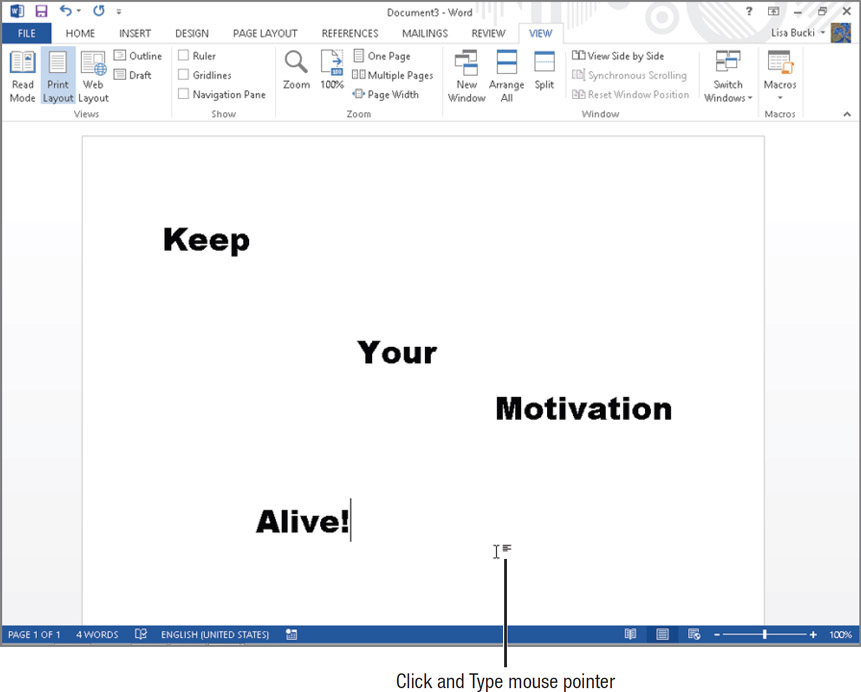
\includegraphics[scale=0.4]{dennis-grafik/word2.jpg}
	\caption{Arbetsytan i Word 2013 (måste kolla om jag får använda bilden)}\label{fig:word2}	
\end{figure} 

